\section{Monte Carlo event generation}
\label{sec:mc}

We used the external model interface in MadGraph~\cite{madgraph} 
to generate $pp \to tt$ and $pp \to ttj$ events at LO 
with the Lagrangian described in Equation \ref{eqn:L_berger} with $f_L = 0$, $f_R = 1$.  
Different values of $f_R$ were modelled by rescaling the cross-sections
for the t-channel (Fig.~\ref{fig:tchannel}) and s-channel (Fig.~\ref{fig:schannel}) 
by $f_R^4$ and $f_R^2$, respectively.
The range of $Z'$ masses considered was 100 GeV to 2 TeV in the t-channel
and 200 GeV to 2 TeV in the s-channel. 
The minimum mass cut is higher for the s-channel where
the $Z'$ boson decays to a top and a light flavour quark
to ensure the on-shell $Z'$ mass is always  larger than the top mass.
Note that we generated two events with two distinct MadGraph settings for
the simulation of top decays: in the first case the decay was handled 
by Pythia, and in the second case by the {\tt DECAY} package within
MadGraph, which does a better job at taking the spin information into
account.

We used the CTEQ6L~\cite{cteq6l} parton distribution function (PDF)
and set the renormalization and factorization scales
to be at the top mass scale ($m_{t} = 172.5$ GeV). 
The width of the $Z'$ boson was calculated using 
BRIDGE~\cite{bridge} and verified the results with MadGraph~\cite{madgraph}. 
The generated events were fed to Pythia for 
parton showering.
The detector response was taken into account with the standard CMS
fast-simulation program.

The total production cross sections for $tt$ and $ttj$ 
at the leading-order (LO) are shown as a function of $Z'$ 
mass in Fig.~\ref{fig:sstopcross}. 
Our calculated cross sections agree well with the 
published literature~\cite{berger}. 

\begin{figure}[htb]
\begin{center}
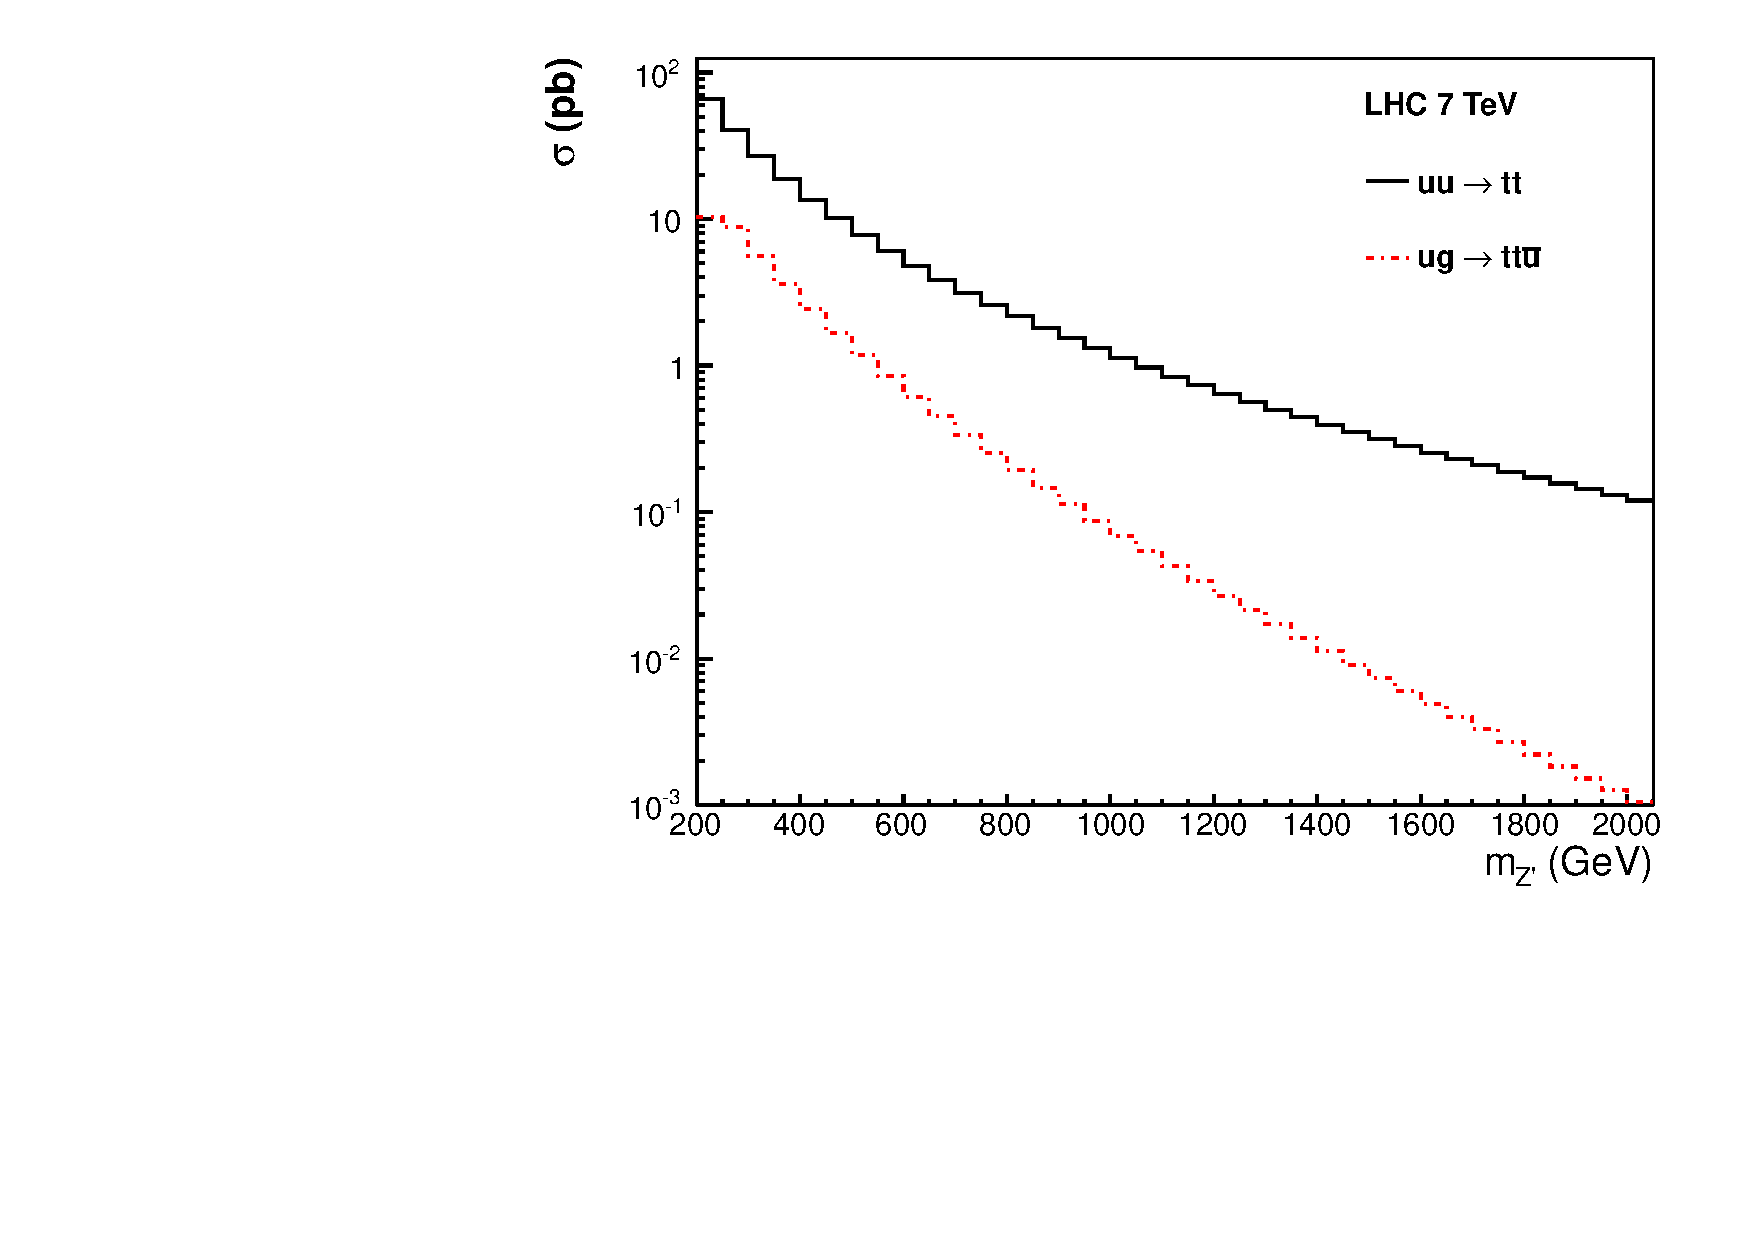
\includegraphics[width=0.7\linewidth]{figs/sstopcross.pdf}
\caption{ LHC production cross section for $tt$ and $ttj$ diagrams using right-handed coupling, $f_R = 1$. 
The renormalization and factorization scales are set to the top mass. \label{fig:sstopcross}}
\end{center}
\end{figure}